\section{The Architect's Question}\label{the-architects-question}

After this chapter we should be able to walk into a running inference
system, read its metrics, and answer a deceptively hard question:
\emph{is this system meeting its obligations, and if not, which lever do
we pull?} Most serving teams instrument the wrong thing --- model
capability and offline quality --- and then are blind when a real
workload misbehaves. This chapter builds the metric hierarchy that turns
raw telemetry into architecture decisions: what to log, what each number
means, how to read a latency \emph{distribution} instead of a mean, and
how to tell bandwidth-bound from compute-bound purely from the counters.
After this chapter, ``the system felt slow'' becomes a falsifiable,
diagnosable claim.

\section{Concept}\label{concept}

\subsection{The Metric Hierarchy}\label{the-metric-hierarchy}

Not all numbers are equal. We organize serving telemetry into three
layers, each answering a different question and each consumed by a
different role:

\begin{enumerate}
\def\labelenumi{\arabic{enumi}.}
\item
  \textbf{Workload metrics} --- what the system is being \emph{asked} to
  do. Requests per second (rps), the token profile (input length, output
  length, context length), and concurrency. These are the independent
  variables; we do not control them, we characterize them. For the
  canonical enterprise-Q\&A RAG workload these are fixed by §14:
  \textasciitilde10 rps average with \textasciitilde40 rps peaks,
  \textasciitilde9,200 input + \textasciitilde300 output tokens per
  request, TTFT 1.2 s / TPOT \textasciitilde25 ms.
\item
  \textbf{Serving metrics} --- how \emph{well} the system performs under
  that workload. Time-to-first-token (TTFT), time-per-output-token
  (TPOT), inter-token latency, and \textbf{goodput} (tokens produced
  that actually meet the SLO). These are the dependent variables; they
  are what the SLO is written against.
\item
  \textbf{Resource metrics} --- \emph{why} performance is what it is.
  HBM bandwidth utilization, FLOP utilization / model FLOPs utilization
  (MFU), KV-cache occupancy, memory pressure, and queue depth. These
  reveal the binding constraint.
\end{enumerate}

The discipline this chapter works toward: \textbf{never jump from a
workload metric straight to a resource metric.} The causal chain is
\emph{workload → serving → resource}. A slow response (serving) is
diagnosed by asking whether the kernel is bandwidth- or compute-bound
(resource), which is only meaningful given the token profile (workload).
Skipping a layer produces superstition --- ``it's slow, let's buy GPUs''
--- instead of a mechanism.

\begin{figure}
\centering
\pandocbounded{\includegraphics[keepaspectratio,alt={\hyperref[fig:6.1]{Fig 6.1} --- The metric hierarchy as a diagnostic chain {[}ILLUSTRATIVE conceptual{]}},width=\maxwidth{\textwidth},keepaspectratio]{figures/fig-06-0601.pdf}}
\caption{\hyperref[fig:6.1]{Fig 6.1} --- The metric hierarchy as a diagnostic chain
{[}ILLUSTRATIVE conceptual{]}}

\label{fig:6.1}\end{figure}

\emph{\hyperref[fig:6.1]{Fig 6.1} --- The three metric layers and the top-down diagnostic
path from a p95 TTFT breach to its root cause. Causation runs bottom-up
(resource → serving → workload); diagnosis runs top-down.}

\subsection{Why the Wrong Metric
Persists}\label{why-the-wrong-metric-persists}

Teams default to measuring what they already have dashboards for: model
quality (accuracy, ROUGE, benchmark scores) and average latency. Both
are dangerously incomplete. Quality is the \emph{goal} but never the
\emph{bottleneck}; average latency is a single scalar that hides the
tail that actually violates SLAs. The entire thesis of this chapter is
that the metric that drives an architecture decision is usually
\textbf{not} the metric the model card advertises.

\section{Mental Model}\label{mental-model}

Think of the three metric layers as a \textbf{diagnostic chain}, like
the layers of the OSI stack in miniature:

\begin{itemize}
\tightlist
\item
  \textbf{Workload} is the \emph{traffic} --- what we are asked to do.
\item
  \textbf{Serving} is the \emph{service} --- how well we did it.
\item
  \textbf{Resource} is the \emph{engine} --- how hard the machine is
  working, and on what.
\end{itemize}

When something breaks, we read top-down: a p95 TTFT breach (serving)
forces us to look at the token profile (workload: did context length
grow?) and then the resource layer (resource: is prefill queuing because
we're FLOP-bound?). When the numbers are healthy, the chain confirms our
architecture was right.

The mental model also inculcates \textbf{one number naming many
different things}. ``Throughput'' without a qualifier is meaningless: is
it requests per second, tokens per second, or \emph{goodput} --- tokens
per second that arrived before the SLO deadline? We commit to always
qualifying.

\section{Worked Example}\label{worked-example}

\subsection{Latency Is a Distribution, Not a
Mean}\label{latency-is-a-distribution-not-a-mean}

The single most common measurement error is reporting (and SLO-ing) the
\emph{average} latency. Consider a request stream where 99\% of requests
complete in 0.8 s but 1\% take 5 s. The mean is

\[
\mathbb{E}[L] = \sum_i p_i \cdot L_i = 0.99 \times 0.8 + 0.01 \times 5.0 \approx 0.84 \text{ s}
\]

--- looks fine. But under a p95 TTFT SLO of ≤ 2 s, the 99th-percentile
straggler blows the p95 budget the moment the outlier fraction crosses
5\%. Averages wash out the tail; percentiles expose it.

\begin{figure}
\centering
\pandocbounded{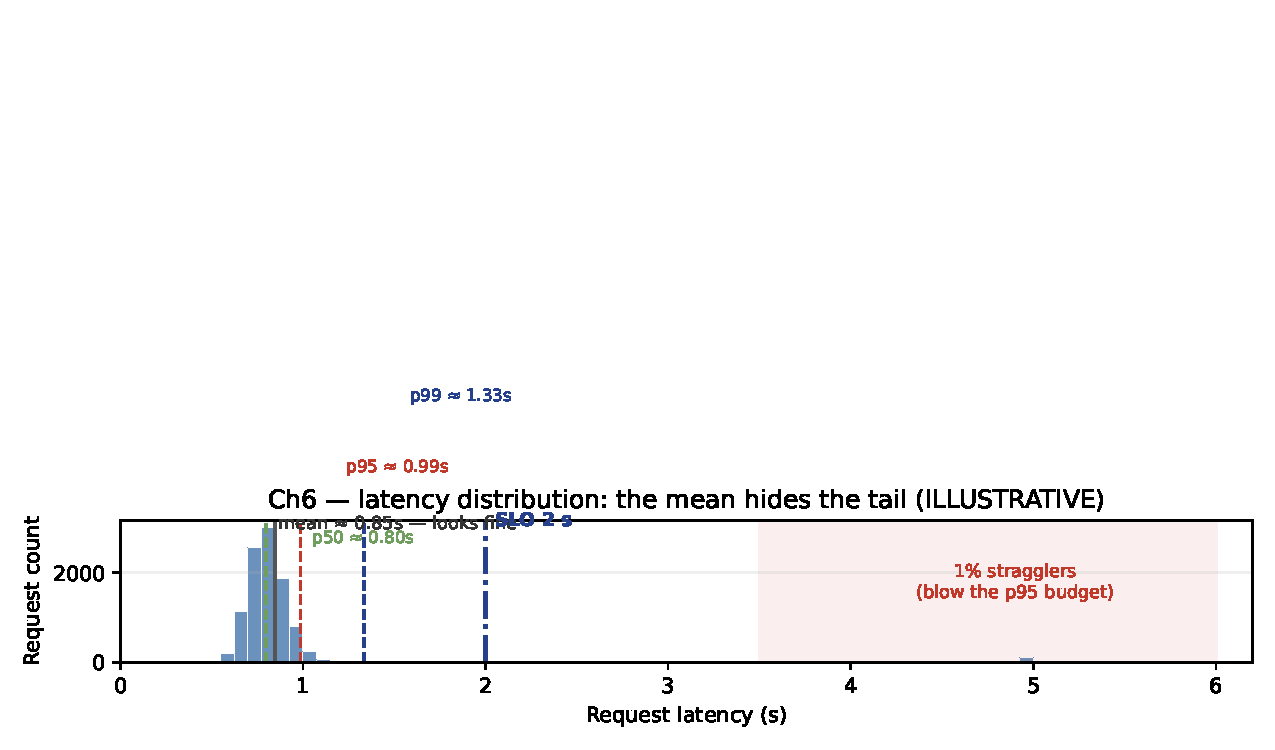
\includegraphics[keepaspectratio,alt={Fig 6.2 --- Request-latency distribution: p50/p90/p95/p99 and the mean. The mean (\textasciitilde0.84 s) hides the 1\% stragglers at \textasciitilde5 s that breach the p95 TTFT budget (ILLUSTRATIVE)},width=\maxwidth{\textwidth},keepaspectratio]{figures/fig-06-0602.pdf}}
\caption{Fig 6.2 --- Request-latency distribution: p50/p90/p95/p99 and
the mean. The mean (\textasciitilde0.84 s) hides the 1\% stragglers at
\textasciitilde5 s that breach the p95 TTFT budget (ILLUSTRATIVE)}

\label{fig:6.2}\end{figure}

\emph{\hyperref[fig:6.2]{Fig 6.2} --- Why the mean is not a signal. The same request stream
of 99\% @ 0.8 s + 1\% @ 5 s reported as a single number looks healthy
(mean ≈ 0.84 s), yet the p95 and p99 paint a very different picture
under a 2 s SLO. Log the distribution; SLO against the percentile.}

Apply this to the canonical workload. We budget TTFT ≤ 1.2 s (retrieval
\textasciitilde120 ms + prefill \textasciitilde1.08 s) with a p95 ≤ 2 s.
Suppose a flash crowd (the \textasciitilde40 rps peak) causes prefill
requests to queue. If on average the batch is well-behaved, p50 TTFT
might sit at \textasciitilde1.0 s. But the jobs that arrive behind 3
same-time prefill requests each pay the full 1.08 s prefill of the job
ahead of them, so p95 TTFT drifts to \textasciitilde2.5 s. The
\emph{average} says ``fine''; the \emph{p95} says ``we just violated our
SLO.'' We hence log p50, p90, p95, and p99 independently and run the SLO
against the percentile, never the mean. {[}2°{]} SLO-derived from the
§14 canonical latency budget; the arithmetic is the point, not a
citation.

\subsection{Goodput vs Raw Throughput}\label{goodput-vs-raw-throughput}

Deploying a higher-throughput configuration can \emph{reduce} goodput.
Concretely: suppose we enable larger dynamic batching to raise raw
tokens/s from 50 tok/s to 70 tok/s, but the batch window pushes p95 TTFT
from 1.8 s to 2.3 s --- above the 2 s SLO. The extra 20 tok/s are
produced, but every one of them misses the deadline. Raw throughput is
up 40\%; \textbf{goodput} (tokens that met the SLO) is effectively
unchanged, because the batch of SLO-compliant tokens didn't grow.
Goodput is the metric the customer experiences; raw throughput is what
the GPU achieves. The architect optimizes goodput. This is why
``faster'' hardware or bigger batches do not trivially mean a better
system.

\subsection{Detecting the Regime: Bandwidth-Bound vs
Compute-Bound}\label{detecting-the-regime-bandwidth-bound-vs-compute-bound}

The most decision-relevant resource question is: is this layer
bandwidth-bound or compute-bound? We recall the arithmetic from \hyperref[chap:2]{Chapter 2}:

\begin{itemize}
\item
  \textbf{Decode is HBM-bandwidth-bound.} Generating one token needs a
  full forward pass over the 70B weights = 140 GB (FP16) of reads per
  token. Within a \textasciitilde25 ms TPOT budget that demands 140 GB /
  0.025 s ≈ \textbf{5.6 TB/s} of HBM bandwidth, against an H100's
  \textasciitilde3.35 TB/s peak {[}2° FACT{]}. 5.6 \textgreater{} 3.35,
  so a single H100 \emph{cannot} meet the budget on bandwidth alone ---
  decode is memory-bound, and the fix is more bandwidth (H200 4.8 TB/s),
  fewer bytes per token (quantization), or fewer weight reads
  (speculative decoding / smaller active params). {[}2° DERIVED{]}
\item
  \textbf{Prefill is compute-bound.} The prefill pass for 9,200 input
  tokens costs ≈ 2 × 70e9 params × 9.2e3 tokens ≈ \textbf{1.29 PFLOP},
  which against the \textasciitilde1.08 s prefill budget implies a
  required rate of ≈ 1.19 PFLOPS --- above an H100's
  \textasciitilde0.989 PFLOPS dense BF16 peak (1.19 \textgreater{}
  0.989), so prefill is FLOP-bound: the machine caps out on compute, not
  memory traffic. {[}2° DERIVED{]}
\end{itemize}

At the resource layer, the tell is utilization: a decode kernel pinned
at \textasciitilde95\% of HBM bandwidth but \textasciitilde30\% of FLOPs
is bandwidth-bound; a prefill kernel with \textasciitilde90\% FLOP
utilization is compute-bound. \textbf{The same hardware, the same model
--- the boundary flips between prefill and decode.} This is precisely
why Splitwise/DistServe (and Mooncake's KV-centric disaggregation) split
prefill from decode onto different pools: the bottleneck-regime
difference justifies it. {[}S4{]}{[}1P{]}

\subsubsection{\hyperref[tab:6.1]{Table 6-1} --- Detecting the bottleneck regime from
resource
telemetry}\label{table-6-1-detecting-the-bottleneck-regime-from-resource-telemetry}

\begin{longtable}[]{@{}
  >{\raggedright\arraybackslash}p{0.2000\linewidth}
  >{\raggedright\arraybackslash}p{0.2000\linewidth}
  >{\raggedright\arraybackslash}p{0.2000\linewidth}
  >{\raggedright\arraybackslash}p{0.2000\linewidth}
  >{\raggedright\arraybackslash}p{0.2000\linewidth}@{}}
\toprule\noalign{}
\begin{minipage}[b]{\linewidth}\raggedright
Phase
\end{minipage} & \begin{minipage}[b]{\linewidth}\raggedright
Demand
\end{minipage} & \begin{minipage}[b]{\linewidth}\raggedright
H100 capacity
\end{minipage} & \begin{minipage}[b]{\linewidth}\raggedright
Verdict
\end{minipage} & \begin{minipage}[b]{\linewidth}\raggedright
Resource tell
\end{minipage} \\
\midrule\noalign{}
\endhead
\bottomrule\noalign{}
\endlastfoot
Prefill (9.2K input) & \textasciitilde1.29 PFLOP & \textasciitilde0.989
PFLOPS BF16 & compute-bound & high FLOP / MFU util, mid bandwidth \\
Decode (per token) & \textasciitilde5.6 TB/s weight read &
\textasciitilde3.35 TB/s HBM & bandwidth-bound & high HBM util, low FLOP
util \\

\label{tab:6.1}\end{longtable}

\emph{(All figures {[}2° FACT{]} hardware / {[}2° DERIVED{]} arithmetic
traced to §14 canonical and \hyperref[chap:2]{Chapter 2}.)}

\subsection{Reading Telemetry Into a
Decision}\label{reading-telemetry-into-a-decision}

A concrete dashboard-read → decision trace. We see: p95 TTFT climbing
(serving), KV-cache hit ratio low (resource: memory), and prefill queue
depth growing (serving). Workload is unchanged. Reading up the chain:
low prefix-cache hit means many independent 9.2K prefixes are being
prefill-processed from scratch on the \textasciitilde40 rps peak ---
each \textasciitilde1.29 PFLOP saturating FLOPs. The decision: enable
prefix / RadixAttention-style caching (SGLang) or Automatic Prefix
Caching (vLLM) so shared retrieved-context prefixes are reused instead
of re-prefilled, cutting effective prefill FLOPs and TTFT.
{[}S3{]}{[}1P{]} Prefix caching is a compute-saving move, not a latency
tuning --- and the telemetry told us that.

\section{Measurement}\label{measurement}

Three practical habits anchor the architect:

\begin{enumerate}
\def\labelenumi{\arabic{enumi}.}
\item
  \textbf{Instrument the hierarchy, not just the app.} Deploy counters
  at all three layers from day one --- rps and token profile (workload);
  TTFT/TPOT/goodput percentiles (serving); HBM bandwidth, FLOP/MFU,
  KV-cache occupancy, queue depth (resource). A system that only logs
  serving metrics cannot tell \emph{why}; one that only logs resource
  metrics cannot tell \emph{what it was asked}.
\item
  \textbf{Always qualify ``throughput.''} rps ≠ tokens/s ≠ goodput. The
  same number, three stories. State the SLO window (p95 ≤ 2 s TTFT)
  before quoting any rate, or the rate is meaningless.
\item
  \textbf{Log the distribution.} Capture p50/p90/p95/p99 for every
  latency metric, and the full token-length distribution (a 32K-tail
  context is a different workload than a 9.2K average). The mean is a
  summary, not a signal.
\end{enumerate}

These habits answer the book's recurring question --- \emph{what would
we actually measure here?} --- with three layers of counters at the
edge, before any architecture decision is committed.

\section{Common Mistakes}\label{common-mistakes}

\begin{itemize}
\tightlist
\item
  \textbf{SLO-ing the average.} A 0.84 s mean hides a 5 s tail. SLO
  against p95/p99, and watch the outlier fraction, not the mean.
\item
  \textbf{Optimizing raw throughput when the SLO windows it.} Bigger
  batches raise raw tokens/s but can push TTFT past its deadline,
  zeroing goodput. Optimize goodput.
\item
  \textbf{Jumping straight to ``buy more GPUs.''} A bandwidth-bound
  decode and a prefill-cost problem need different fixes; without the
  resource layer we guess.
\item
  \textbf{Treating hardware peak as a ceiling we can hit.} H100's 3.35
  TB/s is the theoretical HBM peak; real memory-bound kernels realize a
  fraction of it. Design headroom against real utilization, not the spec
  sheet.
\item
  \textbf{Conflating model-quality metrics with serving metrics.}
  Accuracy is the goal; TTFT is the constraint. A slow, accurate model
  fails its SLO just as surely as a fast, wrong one.
\end{itemize}

\section{Architecture Consequence}\label{architecture-consequence}

The metric hierarchy directly dictates architecture. For the canonical
workload:

\begin{itemize}
\tightlist
\item
  \textbf{Bandwidth-bound decode + compute-bound prefill ⇒ consider P/D
  disaggregation} (Splitwise/DistServe/Mooncake) at scale, because
  squeezing both regimes from one resource pool fights itself.
  {[}S4{]}{[}1P{]}
\item
  \textbf{Repeat-prefix RAG ⇒ enable prefix caching}
  (RadixAttention/APC), which turns repeated 9.2K prefills into cached
  lookups and defends the p95 TTFT against the 40 rps peaks.
  {[}S3{]}{[}1P{]}
\item
  \textbf{KV-cache pressure ⇒ quantize or offload KV.} FP8 KV is ≈54\%
  of BF16 {[}S6{]}{[}1P{]}, and vLLM KV-offloading cuts TTFT by 2--22×
  {[}S6{]}{[}1P{]} --- both are memory-layer fixes the telemetry would
  call for when KV occupancy nears capacity.
\item
  \textbf{Speculative decoding where decode bandwidth is the wall} ---
  DFlash reports \textgreater4.3× over baseline / 1.5× vs native MTP
  {[}S5{]}{[}1P{]} --- because it reduces weight reads per accepted
  token.
\end{itemize}

\section{What We Still Don't Know}\label{what-we-still-dont-know}

\begin{itemize}
\tightlist
\item
  \textbf{Goodput in production is rarely published.} The research
  corpus gives strong qualitative and some quantitative anchors
  (Mooncake 525\% simulated throughput / 75\% more requests
  {[}S4{]}{[}1P{]}, DFlash \textgreater4.3× {[}S5{]}{[}1P{]}), but
  portable end-to-end goodput figures across real enterprise RAG
  workloads remain {[}HYPOTHESIS{]}.
\item
  \textbf{Prefix-cache hit rates in mixed workloads} are
  workload-dependent; the actual reduction in prefill FLOPs from
  APC/RadixAttention for a given document-retrieval distribution is
  {[}VERIFY{]}.
\item
  \textbf{Tail-latency drivers under batching} interact: batch size,
  arrival burstiness, and KV fragmentation each affect p99 differently,
  and their joint effect is {[}HYPOTHESIS{]}.
\end{itemize}

\section{End-of-Chapter Mini-Case}\label{end-of-chapter-mini-case}

An on-call architect is paged: ``the internal Q\&A tool got slow after
lunch.'' The dashboard shows rps at the \textasciitilde40 rps peak
(workload, up from the 10 rps baseline), p95 TTFT at 2.4 s against a 2 s
SLO (serving, breached), and KV-cache occupancy at 85\% with low
prefix-hit ratio (resource, memory/FLOP pressure). Following the chain
rather than guessing, the architect reads: a concurrency spike
(workload) with repeated full 9.2K prefills (low prefix hit) is
saturating prefill FLOPs (compute-bound). The architecture is memory-
and compute-sane at the 10 rps design point but was never sized for the
lunch peak. The fix is not ``buy GPUs immediately'' --- it is to enable
prefix caching to collapse the repeated prefills, which the telemetry
shows will address the actual mechanism. The architect re-checks the
dashboard an hour later: p95 TTFT back under 2 s, goodput restored ---
because they measured the right thing at the right layer.
